\documentclass[a4paper, 12pt]{article}

\usepackage[T2A]{fontenc}
\usepackage[utf8]{inputenc}
\usepackage[english,russian]{babel}
\usepackage{amsmath, amsfonts, amssymb, amsthm, mathtools, graphicx}
\usepackage{wrapfig}
\usepackage{subfig}
\theoremstyle{definition}
\usepackage{cancel}
\newtheorem{exmp}{Пример}[section]
\author{Булинский Андрей Вадимович}
\title{Теория вероятностей. Лекции и Семинары}
\date{\today}
\begin{document}
	\maketitle
	\pagenumbering{gobble}
	\newpage
	\pagenumbering{arabic}
	\tableofcontents
	\newpage
	\section{Лекция 1}
	\subsection{Предмет изучения}
	Теория вероятностей изучает закономерности, присущие случайным явлениям. Неслучайные явления будем называть детерминированными. В курсе будем изучать модели случайных экспериментов.\par
	Модель случайных экспериментов подразумевает:
	\begin{enumerate}
		\item Воспроизводимость (контроль основных факторов).
		\item Непредсказуемость исходов.
	\end{enumerate}
	\subsection{Частотная интерпретация вероятностей}
	Основные понятия:\\
	Имеется серия из $N$ повторений эксперимента.\\
	$A$ – явление (событие), которое может произойти.\\
	$N(A)$ – число экспериментов, когда  произошло.\\
	$\nu_N\left(A\right)=\frac{N\left(A\right)}{N}$ – частота события  в серии из  повторений.\\
	\\
	\paragraph{Свойство стабилизации:}
	Пусть $N_1\gg 1$ и $N_2\gg 1$, то $\nu_{N_1}\left(A\right)\approx\nu_{N_2}\left(A\right)$.\\
	$P\left(A\right)$ – вероятность.
	\subsection{Вероятностное пространство}
	Математической моделью случайного эксперимента является вероятностное пространство. Для упрощения задачи используем математический аппарат теории множеств (и теории мер).\par
	Вероятностное пространство состоит из трех множеств $\left(\Omega, F, P\right)$.
	\begin{enumerate}
		\item Непустое множество $\Omega$ (омéга большое) – всевозможные элементарные исходы эксперимента. Пояснение: Элементарные исходы – простейшие, взаимоисключающие исходы.
		
		\begin{exmp}
		однократное подбрасывание монеты. Комментарий: пример с монеткой крайне популярен как в русскоязычных, так и в англоязычных пособиях, поэтому будем использовать числовые значения для обозначения исходов эксперимента: $\Omega=\left\{\text{Г},\text{Р}\right\}$, $\Omega=\left\{H,T\right\}$, $\Omega=\left\{0,1\right\}$.\\
		Здесь введем понятия мощности множества – числа элементов конечного множества. Обозначение: $\left|\Omega\right|=\#\Omega=2$
		\end{exmp}
		\begin{exmp}
		Эксперимент: $n$ - кратное подбрасывание монеты, $\left(n\in\mathbb {N}\right)$.
		Введем понятие элементарных исходов  (омéга малое).\\
		$\omega\in\Omega$, $\omega=\left(k_1,\dddot{},k_n\right)$, где $k_j\in\left\{0,1\right\};j=\overline{1,N}$. $\omega$ – двоичное $N$-разрядное слово.
		Добавим, что мощность $\Omega$ в данном случае $\left|\Omega\right|=2^N$. В теории вероятностей $\Omega$ – пространство элементарных исходов.
		\end{exmp}
		\begin{exmp}
			$n$-кратное подбрасывание игральной кости: $\omega=\left(k_1,\dddot{},k_n\right)$, где $k_j=\left\{1,2,3,4,5,6\right\}$, тогда $\left|\Omega\right|=6^N$.\\
			Часто на практике нас интересует не конечный результат эксперимента, а ответ на вопрос, удовлетворяет ли этот результат определенным критериям (Простейший пример – попадание стрелка в мишень. Нас интересует не в какую точку попадает снаряд, а в какую область мишени он попадет). Применяем теоретико-множественный аппарат.
		\end{exmp}
	\subsection{Операции над множествами}
	\begin{enumerate}
		\item Теоретико-множественное вычитание: $\Omega \backslash A$.
		\item Дополнение к $A$ в $\Omega$: $\overline{A}:=\Omega \backslash A\equiv A^c$. Будем пользоваться теоретико-множественным аппаратом, но поменяем названия: Множество на Событие, Дополнение на Противоположное событие.
		\begin{figure}[h]
			\centering
			\subfloat[$\omega\in A$ — произошло событие $A$.]{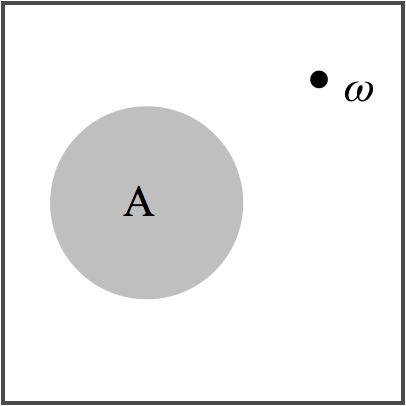
\includegraphics[scale=0.3]{omega_not_in_A.png}}
			\qquad
			\subfloat[$\varnothing \subset A$, $\varnothing\subset B$, $A\cap B=\varnothing$.]{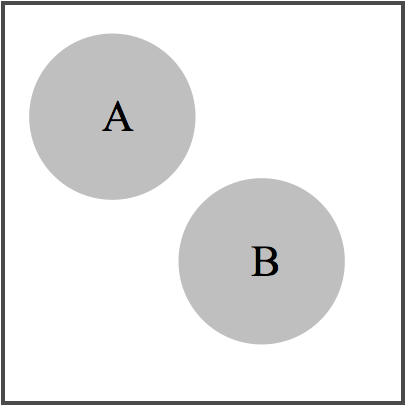
\includegraphics[scale=0.3]{A_and_B.png}}
		\end{figure}
		\par
		$\subset$ – знак нестрогого вложения. $A\subset B$ если $\omega \in A\Rightarrow\omega\in B$, $A=B$ если $\begin{cases}
				A\subset B\\
				B\subset A
				\end{cases}$
		\item Пересечение: $A\cap B=\left\{\omega\in\Omega:\omega\in A, \omega \in B\right\}$.
		\item Объединение: $\omega\in A\cup B\Leftrightarrow$ \{$\omega$ содержится хотя бы в одном из множеств $A$ или $B$\}.
	\end{enumerate}
	\item Выделяется класс $F$ подмножеств $\Omega$, именуемый событиями если:
		\begin{enumerate}
			\item $A\in F \Rightarrow \overline{A}\in F$
			\item $A,B\in F\Rightarrow 
					\begin{cases}
					A\cup B \in F\\
					A\cap B \in F
					\end{cases}$
		\end{enumerate}
		$\Omega\in F$ — достоверные события\\
		$\overline{\Omega}=\varnothing$ — недостоверные события\\
		\subsection{Требования к классу событий:}
		\begin{enumerate}
		\item $\Omega \in F$
		\item $A\in F\Rightarrow \overline{A}\in F$
		\item $A_1,A_2\in F\Rightarrow A_1\cup A_2\in F$
		\item $A_1,A_2\in F\Rightarrow A_1\cap A_2\in F$
		\end{enumerate}
		\paragraph{Замечание:} из первых трех свойств следует четвертое, а из первых двух и четвертого следует третье. Такие свойства подмножеств $\Omega$ называются алгеброй.
		\item На событиях $A\in F$ задается функция $P$ со свойствами, имитирующими свойства частот.\\
		$F\ni A\longrightarrow P\left(A\right)\in\mathbb{R}$\\
		$\nu_N(A)=\frac{N(A)}{N}$, $\nu_N(\Omega)=\frac{N(\Omega)}{N}=\frac{N}{N}=1$\\
		$A_1\cap A_2=\varnothing$\\
		\paragraph{Соглашение:} иногда пишем вместо $A_1\cup A_2\equiv A_1+A_2$ только при условии, что $A_1\cap A_2=\varnothing$.\\
		$N(A_1+A_2)=N(A_1)+N(A_2)$\\
		$\nu_N(A_1+A_2)=\nu_N(A_1)+\nu_N(A_2)$\\
		\subsection{Свойства функции $P$}
		\begin{enumerate}
		\item $P(A)\ge 0$
		\item $P(\Omega)=1$
		\item $P\left(A_1\cup A_2\right)=P(A_1)+P(A_2)$, если $A_1\cap A_2=\varnothing$.
		\end{enumerate}
		\subsection{Счетная аддитивность}
		Если $\left\{A_n\right\}^\infty_{n=1}\subset F$ и $A_i\cap A_j=\varnothing, i\ne j$, то 
		\begin{equation}
			P\left(\bigcup^\infty_{n=1}A_n\right)=\sum_{n=1}^\infty P\left(A_n\right)
		\end{equation}
	\end{enumerate}
	\section{Семинар 1}
	\textit{Задача о выборках (вспомогательная)}\par
	Есть совокупность $N$ различных объектов $\left(N\in\mathbb{N}\right)$, причем занумерованных.
	\begin{equation*}
		\begin{matrix}
		\{a_1, & a_2, & a_3, & \dddot{} &, & a_n\} \\
		\updownarrow & \updownarrow & \updownarrow && &\updownarrow\\
		\{1, & 2, & 3, & \dddot{} &, & N\}
		\end{matrix}
	\end{equation*}
	Сколько выборок $n$ из этой совокупности можно привести?
\end{document}
